

%----------------------------------------------------
% CHƯƠNG CƠ SỞ LÝ THUYẾT
%----------------------------------------------------
\chapter{Cơ sở lý thuyết}
\label{chap:co_so_ly_thuyet}
\onehalfspacing % Giãn dòng 1.5


\section{Nền tảng xử lý ảnh và thị giác máy tính}
\label{sec:image_processing_cv_foundation}
Xử lý ảnh (IP) và Thị giác Máy tính (CV) là hai lĩnh vực khoa học kỹ thuật tương hỗ, giúp máy tính thu nhận và diễn giải thông tin trực quan \citep{Gonzalez2018}. IP tập trung vào thao tác tín hiệu ảnh số để cải thiện chất lượng hoặc chuyển đổi biểu diễn, trong khi CV hướng đến việc "hiểu" nội dung ngữ nghĩa của hình ảnh, mô phỏng thị giác người \citep{Szeliski2010}, tích hợp IP với học máy và AI. Đồ án ứng dụng cả hai lĩnh vực.

\textbf{Tiền xử lý ảnh} là giai đoạn then chốt trong hầu hết hệ thống CV, nhằm nâng cao chất lượng và chuẩn hóa dữ liệu đầu vào, từ đó cải thiện hiệu năng toàn hệ thống. Các kỹ thuật phổ biến bao gồm: cắt ảnh (ROI), căn chỉnh hình học, chuyển đổi không gian màu/định dạng, chuẩn hóa kích thước, và lọc/tăng cường ảnh. Thư viện \texttt{OpenCV} cung cấp các thuật toán này và được sử dụng trong đồ án \citep{opencv_library}.

\begin{figure}[H] % [H] để ép ảnh đứng tại vị trí này (cần gói float)
    \centering
    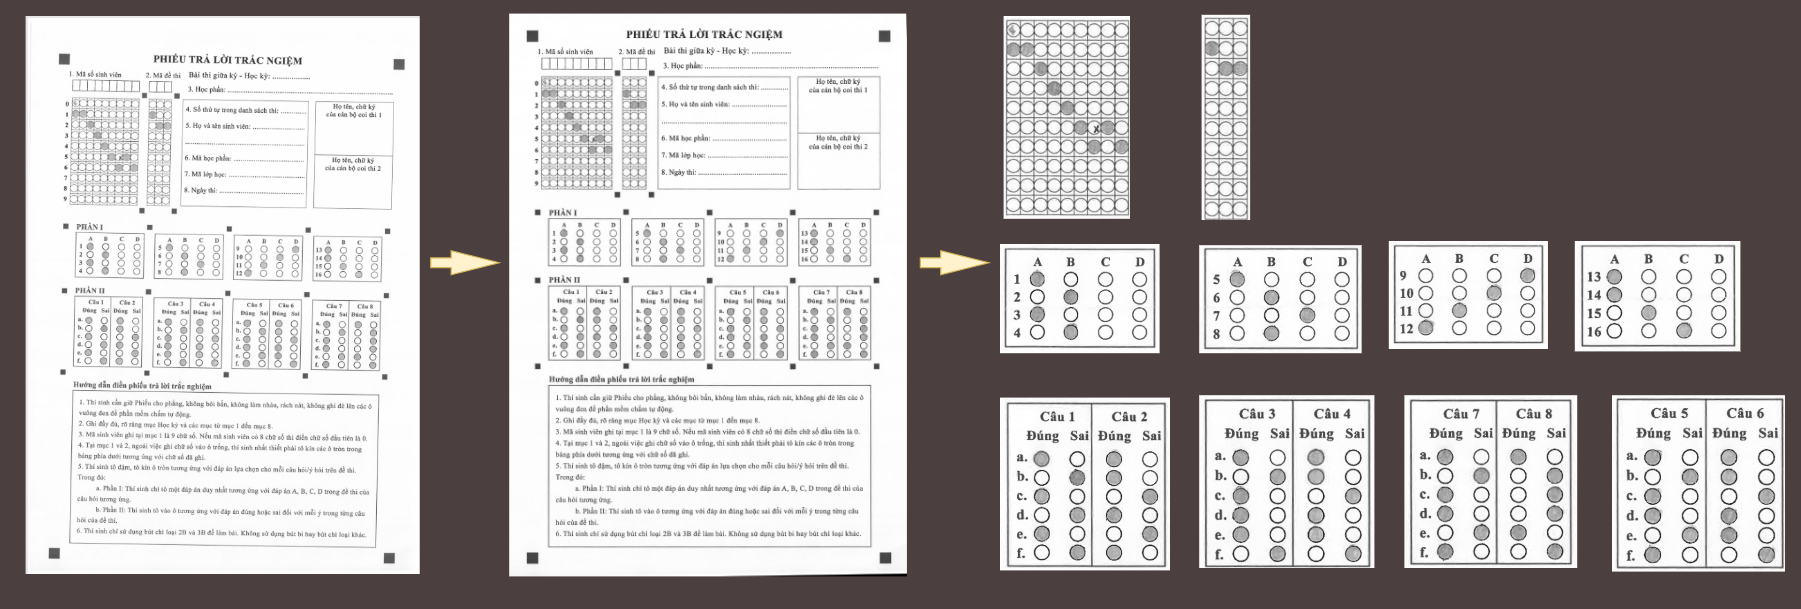
\includegraphics[width=1\textwidth]{img_proj/quy_trinh.png} % Thay bằng đường dẫn ảnh của bạn
    \caption{Minh họa các bước tiền xử lý ảnh tiêu biểu: (a) Ảnh gốc, (b) Ảnh sau khi căn chỉnh, (c) Ảnh sau khi cắt vùng quan tâm và chuẩn hóa.}
    \label{fig:preprocessing_example}
\end{figure}

\section{Nhận diện đối tượng bằng học sâu}
\label{sec:object_detection_dl}
Nhận diện đối tượng là một trong những bài toán cốt lõi và đầy thách thức của thị giác máy tính, với mục tiêu không chỉ phân loại các đối tượng hiện diện trong ảnh mà còn định vị chính xác vị trí của chúng bằng các hộp giới hạn (bounding boxes). Sự phát triển mạnh mẽ của học sâu, đặc biệt là các kiến trúc Mạng Nơ-ron Tích chập (CNNs), đã mang lại những đột phá ấn tượng trong lĩnh vực này, cho phép xây dựng các mô hình có độ chính xác và khả năng tổng quát hóa cao \citep{Goodfellow2016}.

\subsection{Kiến trúc mạng Nơ-ron tích chập (CNN)}
\label{ssec:cnn_architecture}
Mạng Nơ-ron tích chập (CNN) là một lớp chuyên biệt của mạng nơ-ron nhân tạo, được thiết kế để tự động và thích nghi học các phân cấp đặc trưng từ dữ liệu đầu vào có cấu trúc dạng lưới, như hình ảnh \citep{LeCun1998}. Đặc điểm nổi bật của CNN là khả năng chia sẻ tham số (parameter sharing) và cấu trúc phân cấp các tầng, cho phép mạng học được các đặc trưng từ đơn giản (như cạnh, góc) ở các tầng đầu đến phức tạp (như bộ phận của đối tượng) ở các tầng sâu hơn. Một kiến trúc CNN điển hình thường bao gồm:
\begin{itemize}
    \item \textbf{Tầng Tích chập (Convolutional Layer):} Áp dụng các bộ lọc (kernels) để thực hiện phép tích chập, trích xuất các bản đồ đặc trưng (feature maps) cục bộ.

    
    \item \textbf{Hàm Kích hoạt (Activation Function):} Một hàm phi tuyến như ReLU (Rectified Linear Unit) được áp dụng sau tầng tích chập để tăng khả năng biểu diễn của mạng.
    \item \textbf{Tầng Gộp (Pooling Layer):} Giảm chiều không gian của các bản đồ đặc trưng, thông qua các kỹ thuật như max pooling, giúp giảm số lượng tham số, kiểm soát overfitting và tăng tính bất biến đối với các thay đổi nhỏ về vị trí.
    \item \textbf{Tầng Kết nối Đầy đủ (Fully Connected Layer):} Thường nằm ở cuối mạng, thực hiện nhiệm vụ phân loại hoặc hồi quy dựa trên các đặc trưng cao cấp đã được học.
\end{itemize}

\begin{figure}[H]
    \centering
    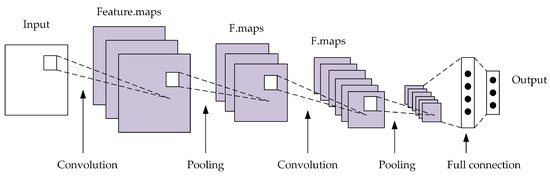
\includegraphics[width=0.85\textwidth]{img_proj/cnn.jpg} % Thay bằng đường dẫn ảnh của bạn
    \caption{Sơ đồ kiến trúc tổng quát của một Mạng Nơ-ron Tích chập (CNN) điển hình, minh họa các tầng chính.}
    \label{fig:cnn_architecture}
\end{figure}

\subsection{Mô hình YOLO (You Only Look Once)}
\label{ssec:yolo_model}

Mô hình YOLO (You Only Look Once) là một kiến trúc mạng nơ-ron tích chập (CNN) tiên tiến, được thiết kế cho bài toán nhận diện đối tượng theo thời gian thực \citep{Redmon2016YOLO}. Điểm khác biệt cơ bản của YOLO so với các phương pháp truyền thống dựa trên vùng đề xuất (region proposal based methods) là cách tiếp cận một giai đoạn (one-stage). Cách tiếp cận này cho phép YOLO thực hiện đồng thời việc định vị và phân loại đối tượng trong một lượt xử lý duy nhất qua mạng, giúp đạt được tốc độ xử lý cao trong khi vẫn duy trì độ chính xác tốt.

Nguyên lý hoạt động cốt lõi của YOLO có thể được tóm tắt qua các bước sau:
\begin{itemize}
    \item \textbf{Chia lưới ảnh:} Ảnh đầu vào được chia thành một lưới các ô (grid cells).
    \item \textbf{Dự đoán trên mỗi ô:} Mỗi ô lưới chịu trách nhiệm dự đoán:
        \begin{itemize}
            \item Một số lượng nhất định các hộp giới hạn (bounding boxes) cùng với điểm tin cậy (confidence score) cho mỗi hộp, phản ánh khả năng ô đó chứa đối tượng và độ chính xác của hộp giới hạn.
            \item Xác suất có điều kiện của từng lớp đối tượng (class probabilities) mà ô đó có thể chứa.
        \end{itemize}
    \item \textbf{Tổng hợp và Hậu xử lý:} Các dự đoán từ tất cả các ô lưới được tổng hợp. Sau đó, một bước hậu xử lý như Non-Maximum Suppression (NMS) thường được áp dụng để loại bỏ các hộp giới hạn trùng lặp và chỉ giữ lại các dự đoán tối ưu nhất.
\end{itemize}

Trong khuôn khổ của đồ án, biến thể \textbf{YOLOv8} đã được lựa chọn và triển khai \citep{UltralyticsYOLOv8}. Đây là một trong những phiên bản mới nhất và có hiệu năng cao thuộc gia đình YOLO, kế thừa và cải tiến từ các phiên bản trước với các ưu điểm nổi bật về tốc độ, độ chính xác và tính linh hoạt trong thiết kế.
Cụ thể, mô hình YOLOv8 được ứng dụng để nhận diện và khoanh vùng các thực thể thông tin quan trọng trên phiếu trắc nghiệm, bao gồm các vùng chứa lựa chọn câu trả lời. Việc huấn luyện, đánh giá và triển khai mô hình YOLOv8 được thực hiện thông qua thư viện \texttt{Ultralytics YOLO}, một nền tảng hiệu quả dựa trên framework học sâu \texttt{PyTorch}.

\begin{figure}[H] % Sử dụng [htbp] để LaTeX tự chọn vị trí tốt hơn, hoặc [H] từ gói 'float' để ép vị trí
    \centering
    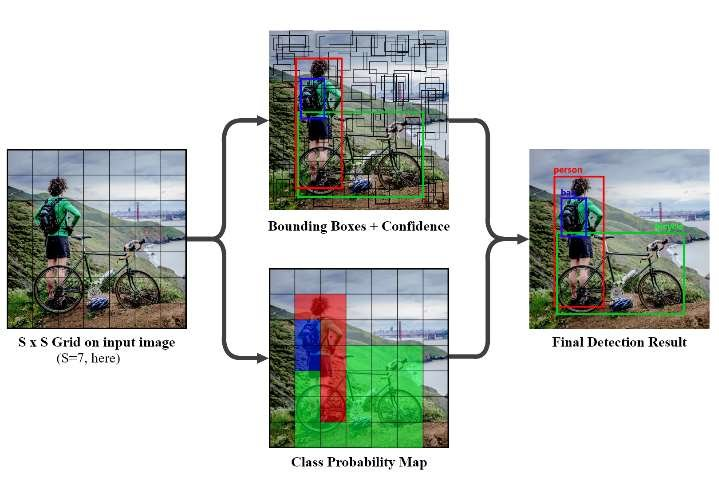
\includegraphics[width=0.7\textwidth]{img_proj/yolo.png} % <<< THAY BẰNG ĐƯỜNG DẪN ẢNH THỰC TẾ CỦA BẠN
    \caption{Minh họa mô hình yolo.}
    \label{fig:yolo_grid_example}
\end{figure}
\section{Xử lý dữ liệu và hậu xử lý}
\label{sec:data_postprocessing}
Kết quả thô từ các mô hình nhận diện đối tượng, mặc dù chứa đựng thông tin giá trị, thường cần trải qua các bước xử lý và hậu xử lý bổ sung. Mục tiêu của các bước này là để tinh lọc, cấu trúc hóa và chuyển đổi dữ liệu thành dạng thông tin hữu ích, sẵn sàng cho các tác vụ tiếp theo như phân tích hoặc ra quyết định trong hệ thống.


\subsection{Phân cụm K-means (K-means Clustering)}
\label{ssec:kmeans_clustering}
K-means là một thuật toán phân cụm (clustering) không giám sát thuộc nhóm phương pháp dựa trên centroid, được sử dụng rộng rãi để phân chia một tập hợp N điểm dữ liệu thành K cụm (clusters) riêng biệt \citep{MacQueen1967}. Mục tiêu cốt lõi của K-means là tối thiểu hóa tổng phương sai trong mỗi cụm, tương đương với việc tối thiểu hóa tổng bình phương khoảng cách Euclidean từ mỗi điểm dữ liệu đến tâm (centroid) của cụm mà nó được gán vào. Quy trình hoạt động của thuật toán K-means diễn ra lặp đi lặp lại qua các bước:
\begin{enumerate}
    \item \textbf{Khởi tạo:} Chọn K tâm cụm ban đầu, có thể là các điểm dữ liệu ngẫu nhiên hoặc thông qua các phương pháp khởi tạo tiên tiến như K-means++.
    \item \textbf{Bước Gán:} Gán mỗi điểm dữ liệu vào cụm có tâm gần nhất.
    \item \textbf{Bước Cập nhật:} Tính toán lại vị trí tâm cho mỗi cụm dựa trên trung bình của tất cả các điểm dữ liệu thuộc cụm đó.
    \item \textbf{Hội tụ:} Lặp lại bước 2 và 3 cho đến khi vị trí các tâm cụm không còn thay đổi đáng kể hoặc đạt đến số vòng lặp tối đa.
\end{enumerate}
Trong bối cảnh dự án, thuật toán K-means (triển khai thông qua thư viện \texttt{Scikit-learn} \citep{scikit-learn}) được ứng dụng để tổ chức và nhóm các hộp giới hạn của các lựa chọn đáp án đã được mô hình YOLO nhận diện. Chẳng hạn, dựa trên tọa độ y, K-means có thể phân cụm các lựa chọn thành các hàng ngang tương ứng, giúp tái tạo cấu trúc logic của phiếu trả lời.

\begin{figure}[H]
    \centering
    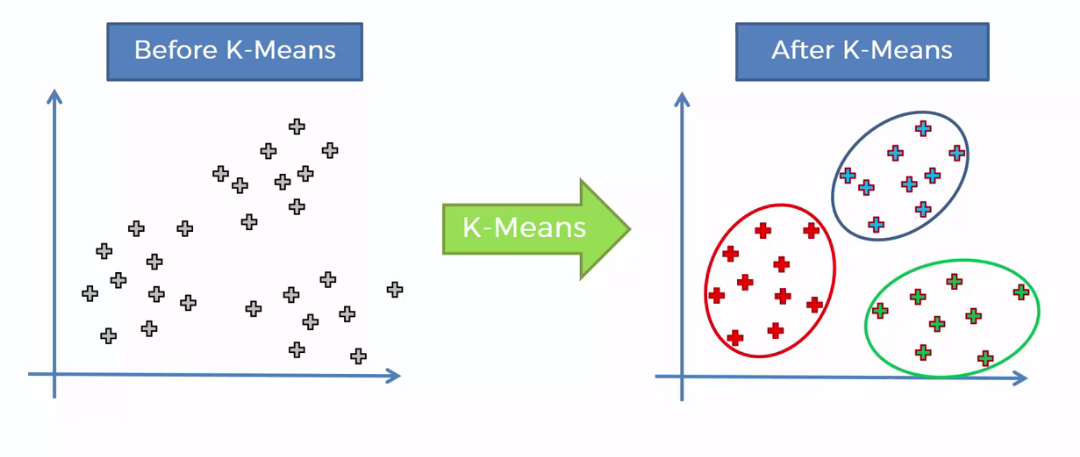
\includegraphics[width=0.75\textwidth]{img_proj/kmean.png} % Thay bằng đường dẫn ảnh của bạn
    \caption{Minh họa ứng dụng K-means để phân cụm}
    \label{fig:kmeans_example}
\end{figure}


%-----------------------------
\subsection{Đối sánh mẫu (Template Matching)}
\label{ssec:template_matching_concise_with_formula}
Đối sánh mẫu (Template Matching) là một kỹ thuật xử lý ảnh cơ bản, nhằm định vị sự xuất hiện của một ảnh mẫu (template) bên trong một ảnh nguồn lớn hơn. Quá trình này bao gồm việc trượt ảnh mẫu qua ảnh nguồn và tính toán một độ đo tương đồng tại mỗi vị trí, tạo ra một bản đồ đáp ứng (response map). Các cực trị trên bản đồ này chỉ ra các vị trí có khả năng cao chứa đối tượng mẫu.

\subsubsection{Độ đo Tương đồng và Phát hiện}
Trong đồ án, Tương quan Chéo Chuẩn hóa (Normalized Cross-Correlation - NCC) được sử dụng để đánh giá mức độ tương đồng. NCC có khả năng kháng tốt với các thay đổi tuyến tính về độ sáng và giá trị của nó dao động trong khoảng $[-1, 1]$. Công thức tính NCC là:
\begin{equation}
R_{NCC}(x,y) = \frac{\sum_{x',y'} (T(x',y') - \bar{T})(I(x+x',y+y') - \bar{I}_{x,y})}{\sqrt{\sum_{x',y'} (T(x',y') - \bar{T})^2 \sum_{x',y'} (I(x+x',y+y') - \bar{I}_{x,y})^2}}
\label{eq:ncc_concise}
\end{equation}
Trong đó $T$ là ảnh mẫu, $I$ là ảnh nguồn, $\bar{T}$ và $\bar{I}_{x,y}$ lần lượt là giá trị trung bình của mẫu và vùng ảnh nguồn tương ứng. Phương thức \texttt{cv2.TM\_CCOEFF\_NORMED} của OpenCV, một biến thể của NCC, được sử dụng trong triển khai.

Các vị trí trên bản đồ đáp ứng có giá trị tương đồng vượt một ngưỡng (threshold) xác định được coi là các phát hiện tiềm năng. Để tinh lọc kết quả, kỹ thuật Loại bỏ Vùng không Cực đại (Non-Maximum Suppression - NMS) được áp dụng để loại bỏ các phát hiện dư thừa cho cùng một đối tượng. Hàm \texttt{findSquares} trong mã nguồn thực hiện chức năng này.

\subsubsection{Ứng dụng trong phân tích biểu mẫu}
Đối sánh mẫu đóng vai trò then chốt trong việc định vị các điểm mốc hình học (fiducial markers), cụ thể là các ô vuông trên biểu mẫu quét. Việc xác định vị trí các ô vuông này là tiền đề cho:
\begin{itemize}
    \item \textbf{Căn chỉnh Hình học (Geometric Rectification):} Sử dụng vị trí các ô vuông (đặc biệt là các ô vuông lớn ở góc) để ước tính phép biến đổi hình học (homography), qua đó căn chỉnh ảnh quét và loại bỏ biến dạng.
    \item \textbf{Phân định Vùng Quan tâm (Regions of Interest - ROIs):} Các ô vuông giúp xác định ranh giới chính xác của các vùng chứa thông tin như mã số sinh viên, mã đề thi, và các khối câu trả lời.
\end{itemize}

Hệ thống sử dụng các kích thước mẫu khác nhau và điều chỉnh ngưỡng linh hoạt để tăng độ tin cậy trong việc phát hiện điểm mốc.

Với tính đơn giản và hiệu quả trong việc xử lý các đối tượng có hình dạng cố định, đối sánh mẫu là một lựa chọn công nghệ phù hợp cho việc phân tích cấu trúc và tiền xử lý các biểu mẫu chuẩn hóa trong dự án này.

\begin{figure}
    \centering
    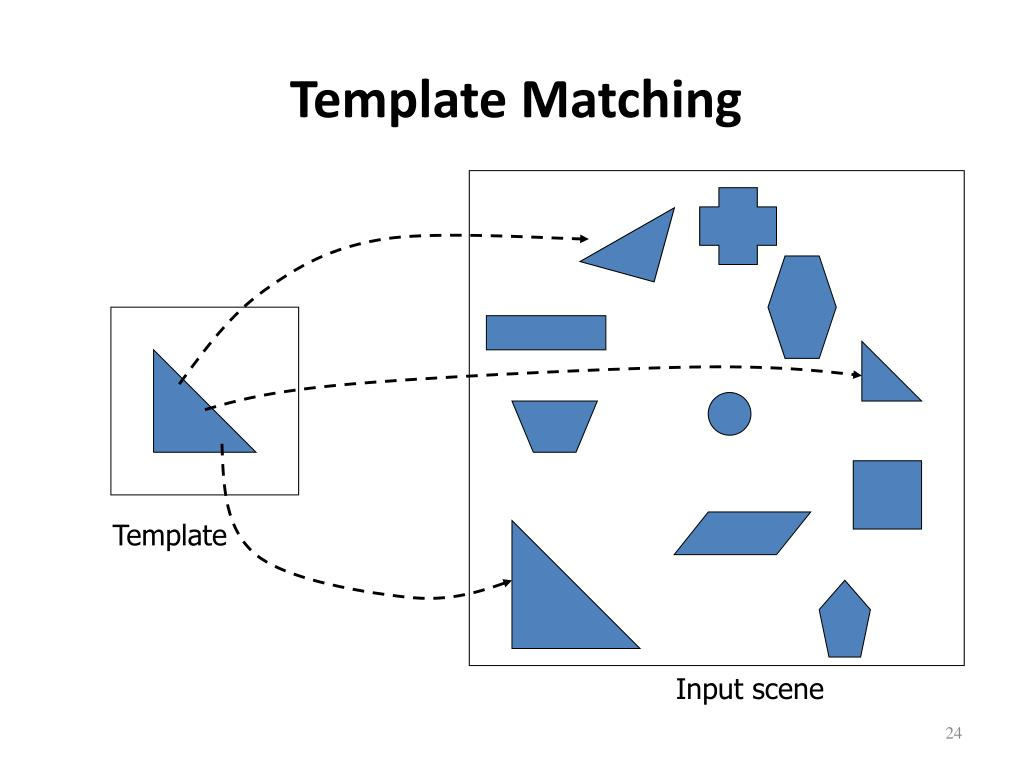
\includegraphics[width=0.8\linewidth]{img_proj/template-matching.jpg}
    \caption{Ví dụ về template matching}
    \label{fig:enter-label}
\end{figure}

% \subsection{Xử lý dựa trên luật (Rule-based Processing)}
% \label{ssec:rule_based_processing}
% Bên cạnh các phương pháp học máy thống kê, hệ thống xử lý dựa trên luật (Rule-based Systems - RBS) vẫn giữ một vai trò quan trọng trong việc tinh chỉnh kết quả, kiểm soát logic và tích hợp kiến thức chuyên môn vào quy trình ra quyết định. Các luật này thường được xây dựng dựa trên các heuristic, đặc điểm hình học, vị trí tương đối của các đối tượng, hoặc các ràng buộc logic của miền ứng dụng cụ thể.
% Trong dự án này, các quy tắc được định nghĩa và áp dụng nhằm:
% \begin{itemize}
%     \item Lọc bỏ các trường hợp nhận diện sai (false positives) hoặc không liên quan dựa trên các tiêu chí như kích thước, tỷ lệ khung hình, hoặc vị trí không phù hợp.
%     \item Xác định chính xác đáp án được thí sinh lựa chọn trong một nhóm các ô lựa chọn, có thể dựa vào phân tích cường độ điểm ảnh hoặc mức độ tô đậm.
%     \item Thực thi các ràng buộc về tính nhất quán của thông tin, cụ thể là số lượng đáp án được chọn cho mỗi câu hỏi.
% \end{itemize}
% Phương pháp tiếp cận dựa trên luật mang lại tính minh bạch, khả năng diễn giải cao cho các quyết định của hệ thống và cho phép tinh chỉnh linh hoạt dựa trên đặc thù của dữ liệu.

% \bigskip % Thêm một khoảng trống nhỏ trước khi kết thúc chương


